\section{Extreme Programming Explained}
% 2 XP's: 2000 and 200? - differences.
% General introduction to XP2k
Extreme Programming (XP) is a software development methodology created by Kent Beck, and this section is based on his book \textit{Extreme Programming Explained (1999)} \citep{xp:explained}. 
Extreme Programming is supposed to be a lightweight, efficient, and fun approach to developing software.
One of its core points, and one of the reasons we chose XP, is the fact it contains development oriented practices.

\noindent XP is based on the four values \textit{Communication, Courage, Feedback, and Simplicity}, which are implemented through the use of the 12 practices:

\begin{tabularx}{\textwidth}{X X X}
	40-hour Week				 & Coding Standards & Collective Ownership \\
	Continuous Integration	  & Metaphor         	 & On-site Customer     \\
	Pair Programming			& Planning Game		& Refactoring          \\
	Simple Design          		  & Small Releases   	& Testing             
\end{tabularx}

These practices also supports each other (e.g. a coding standard supports pair programming) in such a way it creates a synergistic effect.
The complete map of which practices supports each other can be seen in \Cref{fig:practiceSupport}.
\begin{figure}[H]
	\centering
	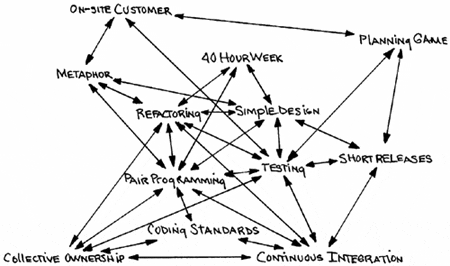
\includegraphics[]{Images/xpPracticeSupport.png}
		\caption{Map of the practices and how they support each other.
			From page 70 in \textit{Extreme Programming Explained (1999)} \citep{xp:explained}. }
	\label{fig:practiceSupport}
\end{figure}

\paragraph{40-hour Week} is the suggested length of a work week in an XP project.
This relative short week is practised because one needs to be on the top of their game when working.
Being well rested and energised should reduce the number of mistakes, as well as increasing patience when pair programming.

\paragraph{Coding Standards} reduces the time it takes to understand code written by others.
A coding standard ensures all developers write code in the same way.
This facilitates refactoring, pair programming, and encourages collective ownership.

\paragraph{Collective Ownership} allows everyone to refactor and review the code.
When no one person owns part of the code, collaboration is enforces while tedious change request are avoided.

\paragraph{Continuous Integration} is used to build the solution several times a day.
This keeps everybody up to date with the latest code changes, avoiding development on fragmented versions.

\paragraph{Metaphor} is used as a shared vision for the project.
The metaphor is used to standardise the names of variables, methods, and classes. 
This standardisation should help to intuitively understand the purpose of the variable, method, or class.

\paragraph{On-site Customer} are a integral role in a XP project.
The on-site customer is responsible for making decisions about priorities and requirements, as well as answering questions.

\paragraph{Pair Programming} is the way to code in a XP project.
It is when two developers work together on the same computer.
While one writes the code, the other analyses and comes with suggestions for improvement.
The development should be seen as a dialogue between the two developers.

\paragraph{Planning Game} is the event where the customer writes user stories, after which, the developers estimates them according to cost.

\paragraph{Refactoring} is the practice used to identify bad smells in the code, e.g. duplicate code, and improve them.

\paragraph{Simple Design} is the best design, and is defined as the easiest that work.
For it to work, it must pass all unit tests and acceptance tests.
Further the best design should be so simple it never has any duplicate code.


\paragraph{Small Releases} are small and frequently versions of the software, which are tested by the customer.
These releases does incrementally complete the system.

\paragraph{Testing} is a mindset, in which, unit tests are developed before the code (Test-Driven Development).
Testing also refers to how the stories and releases are not complete before they pass their respective tests.

%http://www.techrepublic.com/article/extreme-programming-do-these-12-practices-make-perfect/
